\section{Einleitung}\label{sec:02_01_einleitung}
\noindent
\begin{wrapfigure}{r}{0.35\textwidth}
  \begin{center}
    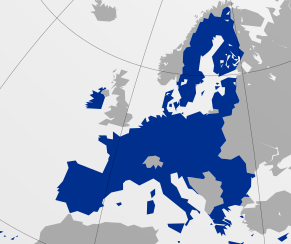
\includegraphics[width=0.35\textwidth]{images/EU_Globe.jpg}
  \end{center}
  \caption{Die EU in Europa}
  \label{fig:EUEuropa}
\end{wrapfigure}
\noindent
Die \textbf{\gls{eu}} ist ein Staatenverbund aus 27 europäischen Ländern (siehe Abb~\ref{fig:EUEuropa}). Außerhalb des geographischen Europas umfasst die EU Zypern (liegt in Asien) und einige Überseegebiete (wie Mayotte). Das Alleinstellungsmerkmal der EU besteht in die \gls{souveraenitaet} der einzelnen Mitgliedstaaten, die aber einige ihrer hoheitlichen Befugnisse in Bereichen bündeln an die EU übertragen. \newline
Diese teilweise Übertragung von Befugnissen an Institutionen, die die Mitgliedstaaten selbst geschaffen haben, bedeutet in der Praxis, dass Entscheidungen zu bestimmten Fragen von gemeinsamem Interesse auf europäischer Ebene demokratisch getroffen werden können. Zu diesen Institutionen gehören:
\newline
\begin{itemize}
  \item das \textbf{europäische Parlament}, das die europäischen Bürgerinnen und Bürger vertritt und direkt von ihnen gewählt wird; (siehe~\ref{subsubsec:EuroParlament})
  \item der \textbf{europäische Rat}, der sich aus den Staats- und Regierungschefs der EU-Mitgliedstaaten zusammensetzt; (siehe~\ref{subsubsec:EuroRat})
  \item der \textbf{Rat}, der die Regierungen der EU-Mitglied-staaten vertritt  (siehe~\ref{subsubsec:Rat}), und
  \item die \textbf{europäische Kommission}, die die Interessen der EU insgesamt wahrt  (siehe~\ref{subsubsec:EuroKommission}).
\end{itemize}
\noindent
Die EU hat insgesamt etwa 450 Millionen Einwohner. Gemessen am Bruttoinlandsprodukt ist der EU-Binnenmarkt der größte gemeinsame Wirtschaftsraum~\cite{wirtschaftsraumEU} der Erde. Die EU stellt eine eigenständige Rechtspersönlichkeit~\cite{rechtpersoenlichkeitEU} dar und hat daher Einsichts- und Rederecht bei den Vereinten Nationen~\cite{vereinteNationen}.\newline
Bis zum 30. Januar 2020 war das vereinigte Königreich teilt der EU und entsprechend war die Anzahl der Mitglieder 28. Am 31. Januar 2020  tratt der Brexit in Kraft und somit wurde diese Mitgliederzahl auf 27 zurückgebracht~\cite{brexitDatum}. Wie hat sich die EU seit ihrer Gründung verändert? Wann und warum wurde die Union überhaupt gegründet? Welche Länder gehören tatsächlich zur EU? Diese und weitere Fragen zur EU werden in den nächsten Kapiteln angegangen.